\documentclass[a4paper, 10pt, onecolumn]{IEEEtran}

\usepackage{graphicx} 
\usepackage{tabularx}
\usepackage{tabulary}
\usepackage{url}       
\usepackage{amsmath} 
\usepackage{amsfonts}
\usepackage{amssymb}
\usepackage{textcomp}
\usepackage{gensymb}
\usepackage{float}
\usepackage[hidelinks]{hyperref}
\usepackage[spanish]{cleveref}
\usepackage{listings}
\usepackage{titlesec} % For custom section titles

% Configuration for code listings
\lstset{
  language=C++,
  basicstyle=\ttfamily\footnotesize,
  stepnumber=1,
  tabsize=2,
  breaklines=true,
  frame=single,
  captionpos=b
}

% Rename listing components
\renewcommand{\lstlistingname}{Fragmento}
\crefname{lstlisting}{Fragmento}{Fragmentos}
\Crefname{lstlisting}{Fragmento}{Fragmentos}

% Custom index names
\renewcommand{\contentsname}{Índice}
\renewcommand{\listfigurename}{Índice de Figuras}
\renewcommand{\listtablename}{Índice de Tablas}
\renewcommand{\lstlistlistingname}{Índice de Fragmentos}

% Custom title formats
\titleformat{\section}[block]
{\bfseries\large} % Bold and large size
{\thesection}{1em}{}

% Custom abstract title
\renewcommand{\abstractname}{Resumen}

\begin{document}
  
  \title{Aproximación de PI Utilizando el Método Monte Carlo}
  \author{José Benavente}
  \markboth{Computación Paralela - Facultad de Ciencias Empresariales - Universidad del Bío-Bío}{}
  \maketitle
  
  \newpage
  
  % General index
  \tableofcontents
  
  % Index of Figures
  \listoffigures
  
  % Index of Tables
  \listoftables
  
  % Index of Code Listings
  \lstlistoflistings
  
  \newpage


\begin{abstract}
Este informe describe un algoritmo basado en el método de Monte Carlo para la aproximación del valor de $\pi$. El método utiliza muestras aleatorias dentro de un cuadrado para estimar la proporción de puntos que caen dentro de las cuatro esquinas generadas al colocar un círculo inscrito dentro de dicho cuadrado. El algoritmo se implementa en \texttt{C++} y hace uso de la biblioteca estándar para la generación de números aleatorios. Además, se presenta una optimización paralela del algoritmo utilizando la biblioteca \texttt{OpenMP}, lo que permite distribuir el cálculo en múltiples hilos de ejecución y así mejorar significativamente el tiempo de ejecución para grandes volúmenes de muestras.
\end{abstract}

\section{Introducción}
El número $\pi$ es una de las constantes matemáticas más importantes y aparece en numerosas áreas de las matemáticas, la física y la ingeniería. Sin embargo, calcular $\pi$ con precisión puede ser computacionalmente costoso. El método de Monte Carlo es un enfoque probabilístico que permite obtener una aproximación de $\pi$ usando técnicas de simulación basadas en números aleatorios. En este informe, se presenta un algoritmo que utiliza este método para estimar el valor de $\pi$.

\section{Método de Monte Carlo}
El método de Monte Carlo se basa en generar un conjunto de puntos aleatorios dentro de un espacio conocido (en este caso, un cuadrado de lado 1) y determinar cuántos de esos puntos caen dentro de una región de interés (un cuarto de círculo inscrito en dicho cuadrado). La proporción de puntos que caen dentro del círculo en comparación con el número total de puntos generados nos permite aproximar el valor de $\pi$.

\subsection{Descripción del Algoritmo}
El algoritmo se implementa en C++ y realiza los siguientes pasos:

\begin{itemize}
    \item Se generan dos números aleatorios $x$ e $y$ entre 0 y 1, los cuales representan las coordenadas de un punto en el plano.
    \item Se verifica si el punto $(x, y)$ cae dentro del cuarto de círculo unitario usando la ecuación $x^2 + y^2 \leq 1$.
    \item Se repite este proceso para un número grande de muestras.
    \item La proporción de puntos que caen dentro del círculo se multiplica por 4 para obtener una aproximación de $\pi$, ya que el área del cuadrado es 1 y el área de un cuarto del círculo es $\pi/4$.
\end{itemize}

A continuación, se muestra un extracto del código de la implementación secuencial del algoritmo en el \cref{lst:sequential}.

\begin{lstlisting}[caption={Implementación Secuencial de Monte Carlo en C++}, label={lst:sequential}]
double sequential(long n) {
  int count = 0;
  std::default_random_engine generator;
  std::uniform_real_distribution<double> distribution(0.0, 1.0);
  
  for (long i = 0; i < n; ++i) {
    double x = distribution(generator);
    double y = distribution(generator);
    
    if (x * x + y * y <= 1.0) {
      count++;
    }
  }
  
  return CIRCLE_MULTIPLIER * count / n;
}
\end{lstlisting}

\subsection{Aproximaciones de PI}
Al ejecutar este algoritmo con un número suficientemente grande de muestras, es posible obtener una aproximación precisa del valor de $\pi$. La precisión mejora a medida que se aumenta el número de muestras. A continuación, en el \cref{tab:results} es posible ver algunos resultados obtenidos al ejecutar el algoritmo:

\begin{table}[H]
    \centering
    \begin{tabular}{|c|c|}
    \hline
    \textbf{Número de muestras} & \textbf{Aproximación de $\pi$} \\
    \hline
    1.000 & 3,192 \\
    10.000 & 3,132 \\
    100.000 & 3,1403 \\
    1.000.000 & 3,14032 \\
    \hline
    \end{tabular}
    \caption{Aproximación de $\pi$ con diferentes números de muestras.}
    \label{tab:results}
\end{table}

\section{Propuesta de Paralelización del Algoritmo}
La implementación secuencial del algoritmo Monte Carlo para la aproximación de $\pi$ se puede acelerar aprovechando la capacidad de procesamiento paralelo. En esta sección, se abordan los puntos clave de la paralelización del algoritmo y se propone una implementación paralela.

Para la implementación paralela del algoritmo Monte Carlo se utilizará la biblioteca OpenMP, que permite distribuir el bucle principal entre múltiples hilos. Cada hilo generará sus propios puntos aleatorios y contará cuántos de ellos caen dentro del círculo. Al final del cálculo, los resultados parciales de cada hilo se combinarán para obtener la cuenta total de puntos dentro del círculo y calcular el valor de $\pi$. Este enfoque garantiza una distribución de la carga de trabajo y minimiza la contención de recursos.

\subsection{Identificación de Cuellos de Botella}
El principal cuello de botella en la versión secuencial del algoritmo es la generación y evaluación de puntos aleatorios en el plano. Esta tarea implica una gran cantidad de cálculos repetitivos y es intensiva en cómputo, especialmente a medida que aumenta el número de muestras. Cada punto se genera y evalúa de forma independiente, lo cual representa una oportunidad perfecta para mejorar el rendimiento mediante paralelización.

\subsection{Partes Potencialmente Paralelizables}
La generación de puntos y su verificación para determinar si caen dentro del círculo son tareas independientes entre sí. Esto significa que el cálculo se puede dividir entre múltiples hilos o procesos, sin que el resultado de una iteración afecte a las demás. Por tanto, el bucle principal del algoritmo es altamente paralelizable.


\subsection{Entorno de Experimentación}
Los experimentos se realizaron en un entorno de hardware y software específico para evaluar el rendimiento de las versiones secuencial y paralelizada del algoritmo. A continuación, se detallan las características de este entorno:

\begin{itemize}
  \item \textbf{Hardware:} Procesador Intel(R) Xeon(R) Gold 5118 de 12 núcleos a 2.30 GHz (modo nominal), con 33 MB de caché L3, 24 MB de caché L2 y 768 KB de caché L1d y L1i. La máquina es virtualizada, utilizando KVM como hipervisor, y cuenta con 62 GB de RAM asignada en un entorno de 64 bits.
  
  \item \textbf{Sistema operativo:} Ubuntu 22.04.5 LTS (GNU/Linux 5.10.0-28-amd64 x86\_64)
  
  \item \textbf{Compilador:} GCC versión 11.4.0, con soporte para OpenMP.
  
  \item \textbf{Librerías:} Se utiliza la biblioteca estándar de C++ para la generación de números aleatorios y la biblioteca OpenMP para implementar la paralelización.
  
  \item \textbf{Entorno de desarrollo:} Code::Blocks configurado con targets de perfilado para las versiones secuencial y paralelizada del algoritmo. Las opciones de compilación incluyen `-g` para depuración, `-pg` para generación de perfiles y `-fopenmp` para habilitar la paralelización.
\end{itemize}

Este entorno permite analizar el rendimiento y la escalabilidad de la implementación paralela en comparación con la versión secuencial, evaluando tanto el tiempo de ejecución como la precisión de ambas versiones del algoritmo.

\subsection{Datos de Prueba}
Para analizar el comportamiento de la versión secuencial del algoritmo Monte Carlo, se realizaron pruebas con diferentes cantidades de muestras, variando entre $1000$ y $1.000.000.000$. Estos datos de prueba permiten observar cómo el tiempo de ejecución crece con el número de muestras, proporcionando información relevante sobre la eficiencia del algoritmo. A continuación, se muestran algunos valores utilizados en las pruebas:

\begin{itemize}
  \item $n = 1.000$
  \item $n = 10.000$
  \item $n = 100.000$
  \item $n = 1.000.000$
  \item $n = 10.000.000$
  \item $n = 100.000.000$
  \item $n = 1.000.000.000$
\end{itemize}

Estos valores de $n$ han sido seleccionados para comprender el comportamiento del tiempo de ejecución y la precisión en distintos escenarios.

\subsection{Perfil de los Algoritmos}
Para el análisis de perfil de la versión secuencial, se utilizó la herramienta \texttt{gprof} y se generó un gráfico de distribución de tiempos de ejecución de las funciones. En la \cref{fig:sec_profile} se muestra la imagen obtenida del perfil de las funciones principales.

\begin{figure}[H]
  \centering
  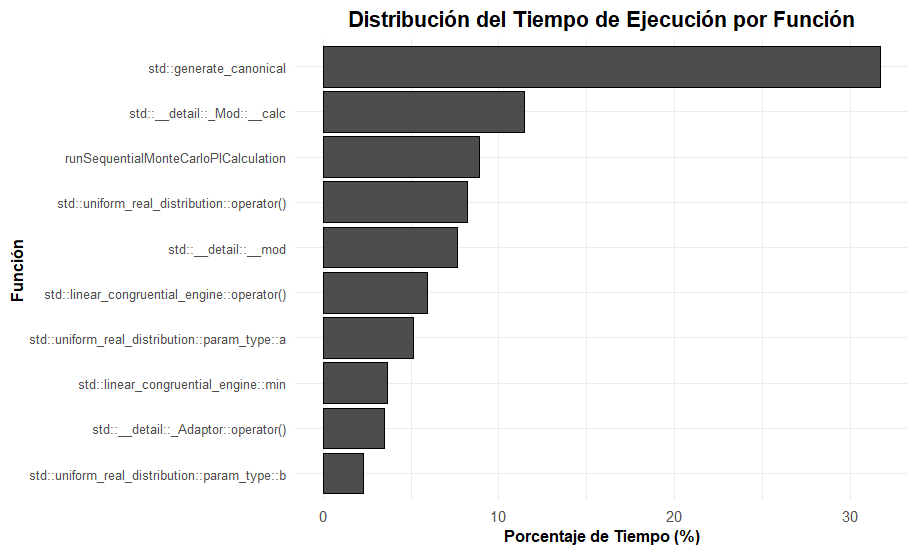
\includegraphics[width=0.8\textwidth]{./img/secuencial_profiling.png}
  \caption{Perfil de tiempo de funciones en la versión secuencial.}
  \label{fig:sec_profile}
\end{figure}

Como se observa en la figura, la función que genera números aleatorios, \texttt{std::generate\_canonical}, es la que más tiempo consume, representando aproximadamente el 31.73\% del tiempo total de ejecución. Las funciones asociadas a la distribución aleatoria, como \texttt{std::uniform\_real\_distribution} y \texttt{std::\_\_detail::\_Mod}, también tienen una participación significativa, representando en conjunto alrededor del 27.6\% del tiempo. La función principal del cálculo secuencial, \texttt{runSequentialMonteCarloPICalculation}, representa cerca del 8.9\% del tiempo de ejecución total.

Es importante destacar que las partes con mayor potencial de paralelización constituyen, en su conjunto, más de un 90\% del tiempo total de ejecución del algoritmo, por lo que estaríamos hablando de que es un problema embarazosamente paralelizable.

\subsection{Muestra de Tiempos de Ejecución}
La siguiente tabla presenta los tiempos de ejecución obtenidos en la versión secuencial del algoritmo para diferentes valores de $n$, calculados en un entorno de experimentación específico. Estos valores muestran el crecimiento en el tiempo de ejecución en función del aumento de muestras, lo que se alinea con el comportamiento esperado del método Monte Carlo.

\begin{table}[H]
  \centering
  \begin{tabular}{|c|c|}
    \hline
    \textbf{Número de muestras ($n$)} & \textbf{Tiempo de ejecución (s)} \\
    \hline
    1.000         & 0,0018318 \\
    10.000        & 0,0115891 \\
    100.000       & 0,0645249 \\
    1.000.000     & 0,576971 \\
    10.000.000    & 5,699076 \\
    100.000.000   & 56,8409 \\
    1.000.000.000 & 573,238 \\
    \hline
  \end{tabular}
  \caption{Tiempos de ejecución en la versión secuencial}
  \label{tab:sequential_execution_times}
\end{table}

\subsection{Conclusiones de la Propuesta de Paralelización}
A partir del análisis del perfil, se identifican algunas funciones que serían candidatas ideales para la paralelización. La función \texttt{runSequentialMonteCarloPICalculation}, que realiza la iteración principal, es altamente paralelizable, ya que cada punto generado es independiente de los demás y no afecta el cálculo de otros puntos. Esto permite distribuir las iteraciones entre múltiples hilos sin introducir dependencias entre las operaciones.

En términos de dependencias, la única dependencia importante se encuentra en la acumulación de la cuenta total de puntos dentro del círculo. Para resolver esto, se puede utilizar una reducción en OpenMP, evitando así el uso de operaciones atómicas que puedan introducir contención y reducir el rendimiento. Por lo tanto y para resumir, se propone dividir las iteraciones del cálculo principal y la generación de puntos aleatorios entre hilos, combinando los resultados parciales al final del cálculo.

\section{Paralelización del Algoritmo}
Como se mencionó en la propuesta de paralelización, se utilizó OpenMP para implementar la versión paralela del método Monte Carlo para el cálculo aproximado de $\pi$. Dicha implementación puede apreciarse a continuación en el \cref{lst:parallel}. Cabe destacar que las pruebas fueron realizadas con 40 hilos de procesamiento.

\begin{lstlisting}[caption={Implementación Paralela de Monte Carlo en C++}, label={lst:parallel}]
double parallel(long n, int num_threads) {
  double step, pi, sum[num_threads];
  
  pi = 0.0;
  step = 1.0 / (double) n;
  omp_set_num_threads(num_threads);
  
  #pragma omp parallel
  {
    double x;
    long i;
    int id;
    
    id = omp_get_thread_num();
    
    for (i = id, sum[id] = 0.0; i < n; i = i + num_threads) {
      x = (i + 0.5) * step;
      sum[id] += 4.0 / (1.0 + x * x);
    }
  }
  
  for (int i = 0; i < num_threads; i++) {
    pi += sum[i] * step;
  }
  
  return pi;
}
\end{lstlisting}

La instrucción \texttt{\#pragma omp parallel} en OpenMP indica que el bloque de código que sigue será ejecutado en paralelo por múltiples hilos. En este caso, el objetivo es dividir las iteraciones de cálculo en el método Monte Carlo entre varios hilos para aprovechar el procesamiento paralelo y reducir el tiempo de ejecución.

Al entrar en la región paralela, cada hilo obtiene un identificador único mediante la función \texttt{omp\_get\_thread\_num()}, el cual se almacena en la variable \texttt{id}. Este identificador permite que cada hilo procese una porción específica del total de iteraciones.

La lógica dentro del ciclo \texttt{for} se adapta para que cada hilo comience en una posición distinta, determinada por su \texttt{id}, y avance en pasos de tamaño igual al número total de hilos, asegurando que las iteraciones no se repitan entre hilos. Cada hilo acumula su propio resultado parcial en el arreglo \texttt{sum}, utilizando su índice correspondiente, \texttt{sum[id]}, para evitar así conflictos de datos entre hilos.

Finalmente, al finalizar la sección paralela, se suman los resultados parciales de cada hilo para obtener el valor aproximado de $\pi$, lo cual se devuelve como resultado de la función.

\subsection{Datos de Prueba}
Para analizar el comportamiento de la versión paralela del algoritmo Monte Carlo, se realizaron pruebas con los mismos datos utilizados al medir el tiempo de ejecución de la implementación secuencial.

\begin{table}[H]
	\centering
	\begin{tabular}{|c|c|}
		\hline
		\textbf{Número de muestras ($n$)} & \textbf{Tiempo de ejecución (s)} \\
		\hline
		1.000         & 0,00276308\\
		10.000        & 0,00292199 \\
		100.000       & 0,0036289 \\
		1.000.000     & 0,00903737 \\
		10.000.000    & 0,0395245 \\
		100.000.000   & 0,253236 \\
		1.000.000.000 & 2,68905 \\
		\hline
	\end{tabular}
	\caption{Tiempos de ejecución en la versión paralela}
	\label{tab:parallel_execution_times}
\end{table}

Al comparar los tiempos de ejecución de la implementación paralela presentados en la \cref{tab:parallel_execution_times} con los tiempos de la implementación secuencial, es evidente que la versión paralela ofrece mejoras significativas en eficiencia para valores grandes de $n$. Esto se debe a que la paralelización permite distribuir las iteraciones del algoritmo Monte Carlo entre múltiples hilos, reduciendo el tiempo total de cálculo.

Para valores de $n$ pequeños, como $1.000$ y $10.000$, la diferencia de tiempo entre las versiones paralela y secuencial es mínima. Esto se debe a que, en estos casos, el tiempo de overhead asociado con la creación y coordinación de múltiples hilos en la versión paralela supera el beneficio obtenido por la división del trabajo. Sin embargo, a medida que $n$ aumenta, la paralelización muestra su ventaja. Por ejemplo, con $100.000.000$ muestras, la versión paralela reduce el tiempo de ejecución a $0,253236$ segundos en comparación con los $56,8409$ segundos de la versión secuencial, representando una mejora sustancial.

En el caso extremo de $1.000.000.000$ de muestras, el tiempo de la implementación paralela es $2,68905$ segundos frente a los $573,238$ segundos de la versión secuencial. Esto evidencia que la paralelización es particularmente efectiva para valores significativamente más grandes, permitiendo una aceleración cercana a $213$ veces en este ejemplo. Estos resultados destacan la efectividad de OpenMP para paralelizar el algoritmo Monte Carlo y reducir los tiempos de ejecución en aplicaciones de cómputo intensivo.

\section{Conclusión}

Los resultados obtenidos en la ejecución de ambas versiones del algoritmo Monte Carlo para el cálculo de $\pi$ permiten analizar la influencia del tamaño de la muestra ($n$) en el tiempo de ejecución y destacar las mejoras alcanzadas mediante la paralelización con OpenMP.

\subsection{Rendimiento de la Versión Secuencial}

En la versión secuencial del algoritmo (ver \cref{tab:sequential_execution_times}), el tiempo de ejecución crece de manera directamente proporcional al tamaño de $n$. Esta proporcionalidad se debe a que cada punto generado requiere una operación independiente de comparación, lo cual significa que al duplicar $n$, el tiempo de ejecución se aproxima también a duplicarse, evidenciando una complejidad temporal lineal, $O(n)$. Esto se observa claramente en el comportamiento de los tiempos registrados, donde el incremento de $n$ lleva a un aumento predecible en el tiempo de ejecución, alcanzando los $573,238$ segundos para $n = 1.000.000.000$. Este comportamiento refleja las limitaciones de procesamiento secuencial en tareas de cálculo intensivo.

\subsection{Mejoras con Paralelización}
Para ilustrar la mejora lograda, podemos calcular el porcentaje de tiempo reducido al comparar ambos métodos:
\[
\text{Reducción de tiempo} = \left(1 - \frac{\text{Tiempo paralelo}}{\text{Tiempo secuencial}}\right) \times 100
\]
Para $n = 1.000.000.000$, este cálculo muestra una reducción de aproximadamente el $99,53\%$, lo cual es particularmente significativo en aplicaciones prácticas que requieren una alta precisión y un número elevado de iteraciones.

A continuación, en la \cref{fig:efficiency}, podemos ver la comparación de tiempos de ejecución entre el algoritmo secuencial y el paralelo.

\begin{figure}[H]
  \centering
  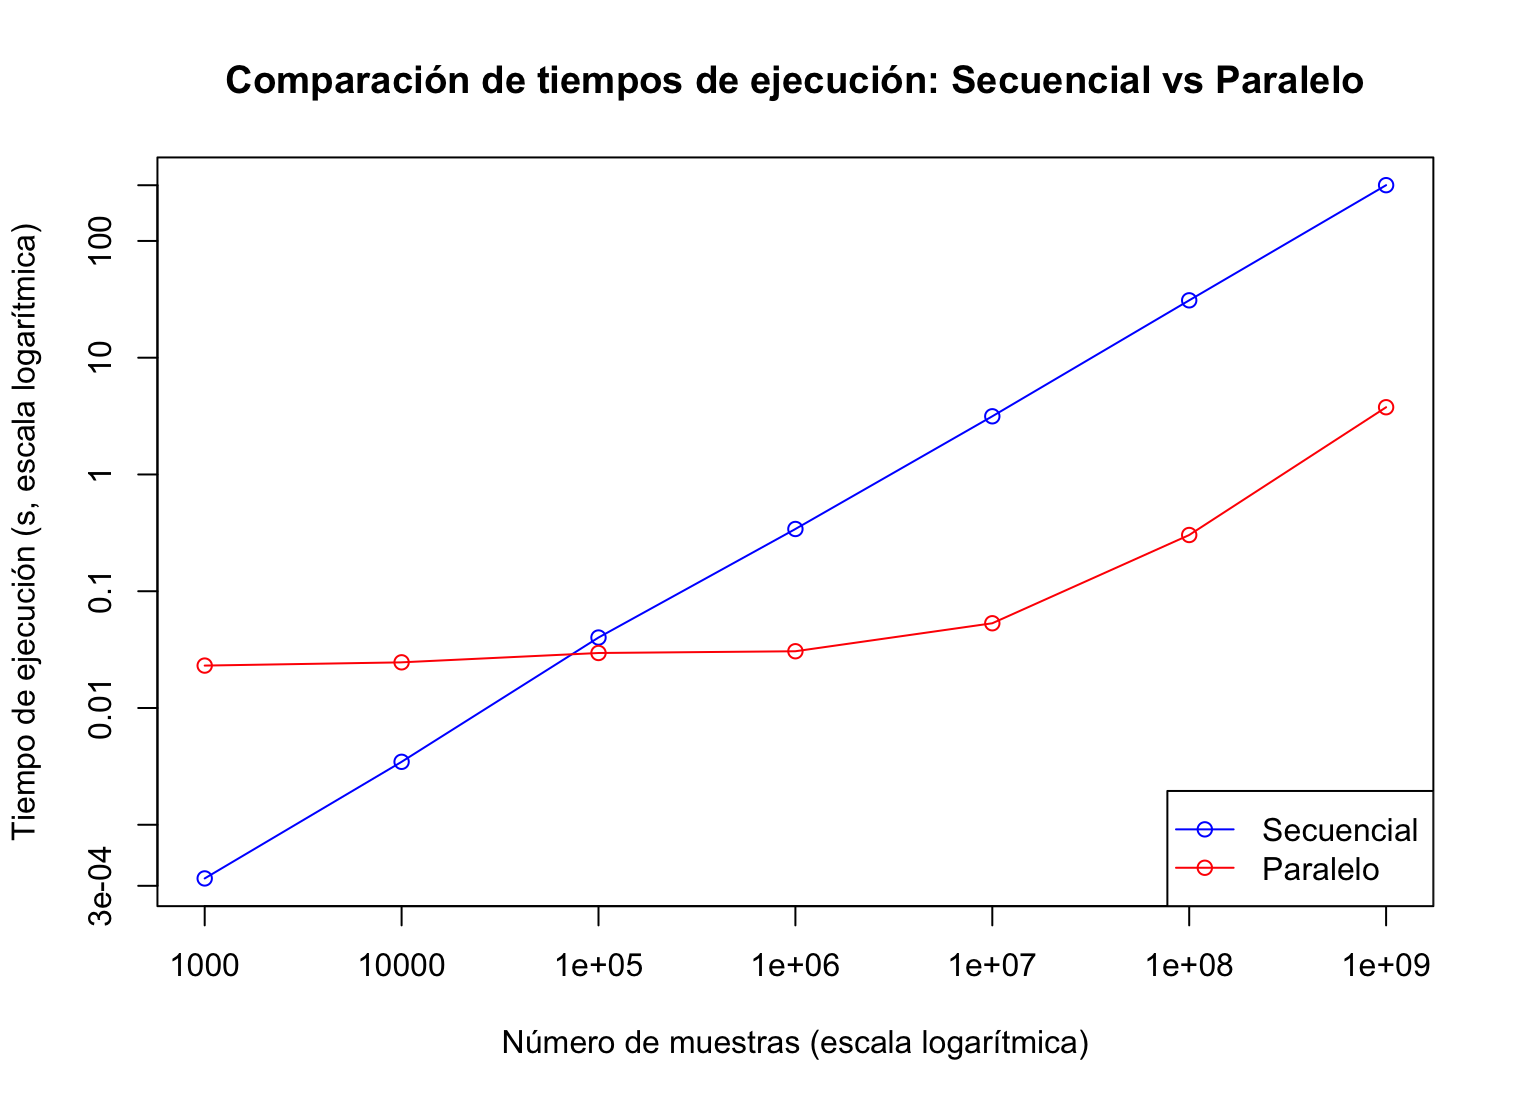
\includegraphics[width=0.8\textwidth]{./img/efficiency.png}
  \caption{Gráfico comparativo de tiempos de ejecución: Secuencial vs Paralelo.}
  \label{fig:efficiency}
\end{figure}

\subsection{Conclusión General}

Estos resultados demuestran la efectividad de la paralelización para acelerar el cálculo del algoritmo Monte Carlo en aplicaciones intensivas de cómputo, alcanzando una eficiencia cercana al máximo teórico en esta configuración. OpenMP, en este contexto, logra optimizar el uso de los recursos de hardware, haciendo posible el cálculo de alto volumen en tiempos considerablemente reducidos.

\end{document}
